\documentclass[12pt,a4paper]{article}
\usepackage[left=2cm,right=2cm,top=2cm,bottom=2cm,bindingoffset=0cm]{geometry}
\usepackage[utf8]{inputenc}
\usepackage[russian]{babel}
\usepackage{cmap}
\usepackage{epigraph}
\usepackage{csquotes}
\usepackage{graphicx}
\graphicspath{ {/} }


\begin{document}

\begin{center}
\hfill \break
\large{МИНОБРНАУКИ РОССИИ}\\
\footnotesize{ФЕДЕРАЛЬНОЕ ГОСУДАРСТВЕННОЕ БЮДЖЕТНОЕ ОБРАЗОВАТЕЛЬНОЕ УЧРЕЖДЕНИЕ}\\ 
\footnotesize{ВЫСШЕГО ПРОФЕССИОНАЛЬНОГО ОБРАЗОВАНИЯ}\\
\small{\textbf{«Санкт-Петербургский государственный
электротехнический университет
	«ЛЭТИ» им. В.И. Ульянова (Ленина)»}}\\
\hfill \break
\hfill \break
 \hfill \break
\hfill\break
\hfill \break
\hfill \break
\hfill \break
\large{Эссе \\

\hfill \break
	по дисциплине: "Экономика"\\
\hfill \break
	Тема: Принцип функционирования электронных денег и криптовалют}\\
\hfill \break
\hfill \break
\hfill \break
\hfill \break
\end{center}
 
\hfill \break
\hfill \break
\hfill \break
\hfill \break
\hfill \break
\hfill \break
\hfill \break
\hfill \break
\hfill \break
\hfill \break
\hfill \break
\hfill \break
\hfill \break
\hfill \break
 
\normalsize{ 
\begin{tabular}{cccc}
Студент гр. 1323 & \underline{\hspace{3cm}} & В.В. Скопцов \\\\
Преподаватель & \underline{\hspace{3cm}} & Т.Н. Лебедева \\\\
\end{tabular}
}\\
\hfill \break
\hfill \break
\begin{center}
	Санкт-Петербург 2022
\end{center}
\thispagestyle{empty} % выключаем отображение номера для этой страницы
 
% КОНЕЦ ТИТУЛЬНОГО ЛИСТА
\newpage 

\tableofcontents

\newpage


\epigraph{A specter is haunting the modern world, the specter of crypto anarchy.}
{\textit{The Crypto Anarchist Manifesto (1988)\\Timothy C. May}}

\section{Введение}

Появление интернета помогло распространению электронных денег в качестве очень практичного и удобного средства оплаты. Быстрота транзакций, защищённость посредством разных криптографических средств и другие достоинства дают огромные преимущества по сравнению с обычными деньгами. Но, в тоже время, на плечи посреднических организаций, которые непосредственно регулируют транзакции, ложится огромная ответственность, которая с дальнейшим развитием и увеличением объёмов цифровых денежных переводов будет только возрастать. Так, например, в распоряжении частных лиц будет находиться всё больше информации о клиентах, что может ставить под угрозу их личную безопасность в случае утечки этих данных. Одним из решений этой проблемы стали криптовалюты, появившиеся относительно совсем недавно. При использовании криптовалют отпадает не только необходимость в стороне осуществляющей транзакцию, но и в государственных эмитентах, из-за чего сама идея децентрализованных платёжных систем подвергается большой критики, в особенности от сторонников государственного контроля за финансами. Но даже если игнорировать политическую сторону вопроса, то остаётся техническая и экономическая, где ещё больше людей найдут недочёты. В данном эссе будут рассматриваться основы функционирования электронных денег и криптовалют в частности, а именно, их устройство и как они представлены в законодательстве РФ.

\section{Определение электронных денег}

Перед тем, как рассмотреть принципы функционирования электронных денег необходимо дать чёткое определение этому достаточно расплывчатому понятию. Для этого можно обратиться к законодательству Российской Федерации.

Федеральный закон «О национальной платежной системе» содержит следующее определение электронных денег 

\begin{displayquote}
	это денежные средства, которые предварительно предоставлены одним лицом (лицом, предоставившим денежные средства) другому лицу, учитывающему информацию о размере предоставленных денежных средств без открытия банковского счёта (обязанному лицу), для исполнения денежных обязательств лица, предоставившего денежные средства, перед третьими лицами и в отношении которых лицо, предоставившее денежные средства, имеет право передавать распоряжения исключительно с использованием электронных средств платежа.
\end{displayquote}

В свою очередь, электронное средство платежа:

\begin{displayquote}
	это средство и (или) способ, позволяющие клиенту оператора по переводу денежных средств составлять, удостоверять и передавать распоряжения в целях осуществления перевода денежных средств в рамках применяемых форм безналичных расчетов с использованием информационно-коммуникационных технологий, электронных носителей информации, в том числе платежных карт, а также иных технических устройств.\cite[статья~3~пункт~18]{cite1} 
\end{displayquote}

\section{Типы электронных денег}

В первую очередь, электронные деньги делятся по принципу физической реализации, а именно, они могут быть либо основаны на \textit{базе смарт-карт}, либо на \textit{базе сетей}. 

Смарт-карты в большинстве случаев представляют из себя пластиковые карты со встроенной микросхемой и операционной системой. Обычные дебетовые или кредитные карты, являются всего лишь средством доступа к счёту, и не могут быть носителями средств, в то время как, смарт-карты непосредственно хранят записи о сумме, которая заложена в них, а так же могут осуществлять криптографические вычисления. Самой известной подобной картой является Visa Cash, разработанная в 1995 году.

Работоспособность электронных денег на базе сетей обеспечивается за счёт некоторой программы, или распределённой сети. Самые известные в России сервисы, работающие по такому принципу являются Яндекс.Деньги и QIWI.

Далее, электронные деньги делятся по принципу государственного регулирования, а именно, на \textit{фиатные} и \textit{нефиатные}.

Фиатные электронные деньги --- это деньги, выраженные в государственной валюте, эмиссия которых происходит по правилам центрального банка. В качестве примера отлично подходит Яндекс.Деньги.

Нефиатные, в свою очередь, эмитируются частными организациями, и не являются гaрaнтированным средством платежа, в отличии от фиатных денег. Самый яркий пример --- платёжный сервис QIWI.

Данное разделение не зависит от технической реализации денег, поэтому деньги могут быть как фиатными, так и нефиатными, вне зависимости от того, какая у них база: сетевая или на основе смарт-карт.

Так же существует разделение на \textit{персонифицированные} и \textit{неперсонифцированные} электронные платёжные средства, которые подразумевают необходимость идентификации и возможность анонимности соответственно.\cite{cite2} 

\begin{figure}[h]
    \centering
    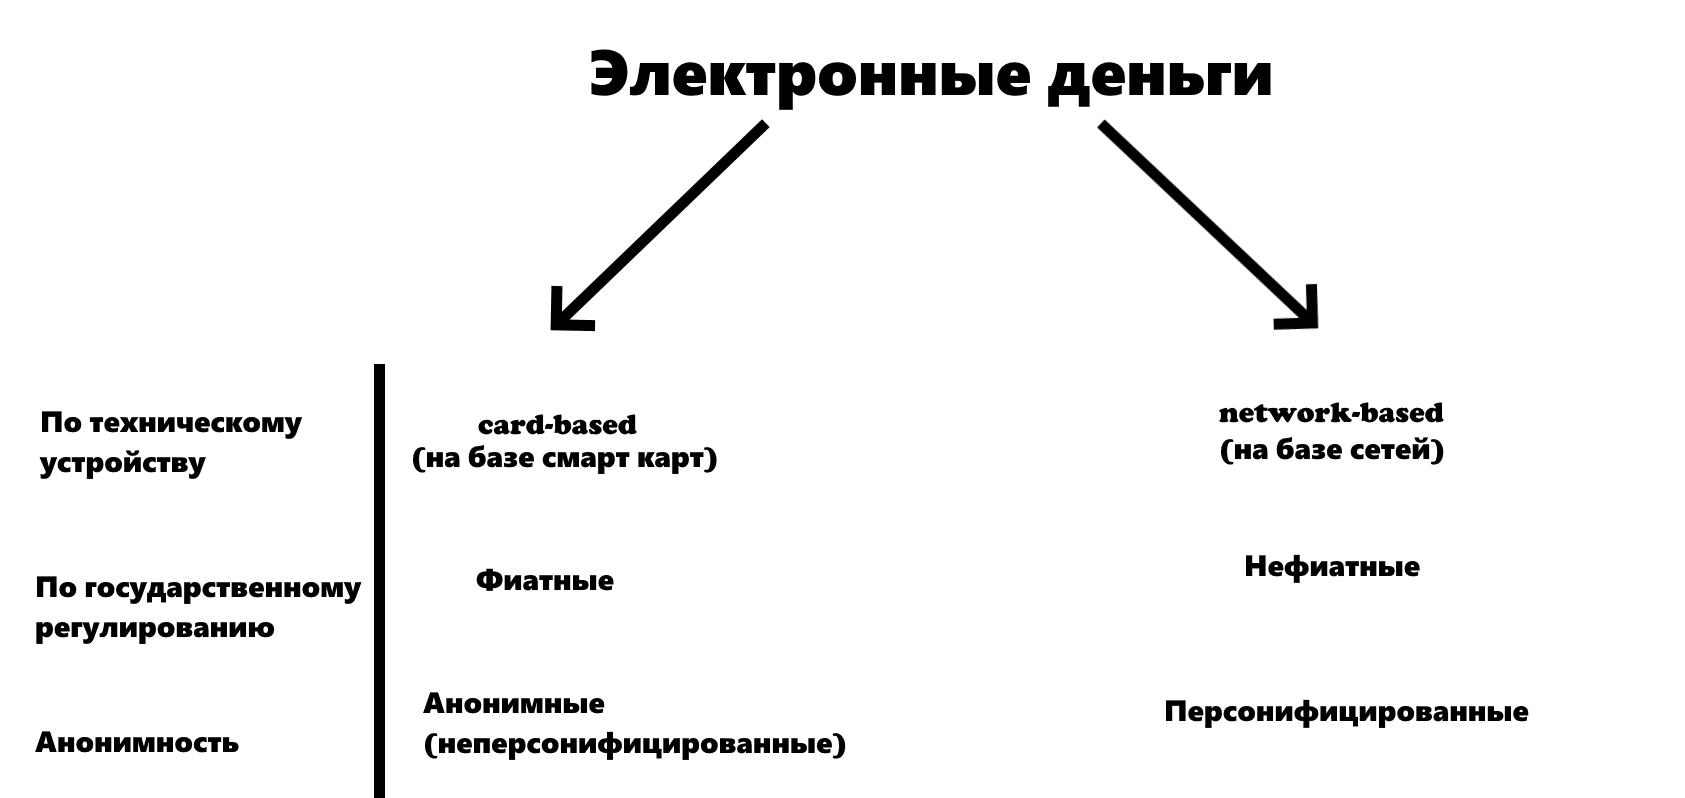
\includegraphics[width=1\textwidth]{pic1}
    \caption{Разделение типов электронных денег.}
    \label{fig:mesh1}
\end{figure}

\section{Теория, обеспечивающая работу электронных денег}

\subsection{Метод слепой цифровой подписи}

В 1982 году вышла работа американского исследователя Дэвида Чаума, где были представлены криптографические методы, которые в последствии легли в основу всех видов электронных платежных систем. Одной из самых важных идей, которые изложил Чаум, была идея слепой цифровой подписи, обеспечивающее следующие возможности, которых не было в стандартных деньгах:

\begin{itemize}
	\item Возможность фиксации факта осуществления транзакции.
	\item Невозможность установления личности получателя третьей стороной.
	\item Возможность остановки транзакции.
\end{itemize}

\subsection{Протокол RSA}

Надёжность транзакций обеспечивается протоколом RSA, который совместно разработали в 1977 году специалисты по информатике Рональд Ривест, Ади Шамир и Леонард Макс Адельман. Устойчивость за счёт фундаментальных криптографических методов позволяет обеспечить анонимность передачи сообщений, из-за чего система RSA стала использоваться во многих сферах в жизни, но особенно важную роль она играет в банковской сфере работая в совокупности с идей слепой цифровой печати.\cite[с.~47]{cite4}



\section{Особенности криптовалют}

Обычные электронные деньги, реализованные на принципах не предполагающих децентрализованное регулирование могут быть уязвимыми за счёт существования третьей доверительной стороны, которая не смотря на использование метода цифровой слепой печати, всё равно полагается на финансовые учреждения. Для решения этой проблемы были созданы определённые методы, в частности, принцип \textbf{доказательство выполнения работы} (англ. proof-of-work), обеспечивающие автономную работу регулирования электронной валюты. Впервые данные методы были использованы в первой криптовалюте Bitcoin, выпущенной в 2009 году в виде открытого программного обеспечения. 

Криптовалюта представляет из себя распределённую базу данных, в которой хранятся общедоступные данные об совершенных транзакциях за весь период её функционирования. За счёт криптографического принципа доказательства выполнения работы система предотвращает слишком частые внесения изменений в базу данных, что предотвращает возможность взлома. Эмиссия происходит во время подтверждений транзакций, обладающих особыми качествами. Со временем, из-за притока новых пользователей сложность проверки историй транзакций в базе данных возрастает и эмиссия становится более дорогой.\cite{cite5}

\subsection{Недостатки криптовалют}

Криптовалюты предоставляют возможность анонимных транзакций, что усложняет возможность госудaрственного регулирования денежных потоков. В частности, анонимность криптовалют позволяет избегать уплату налогов, осуществлять оборот нелегальных товаров.\cite{cite6} 

В рыночной среде часто поднимается вопрос об факте завышения текущих цен криптовалют в сравнении с их гипотетической стоимостью, что основывается на отсутствии внутренней ценности. В частности, лауреат Нобелевской премии по экономике Джеймс Хекман сравнил ажиотаж вокруг биткойна с тюльпаноманией в Голландии в 17 веке.\cite{cite6} Рынок криптовалют действительно напоминает спекулятивный пузырь, к примеру, цена криптовалют может стремительно возрастать за короткий промежуток времени, а потом падать на несколько десятков процентов.

В особенности криптовалюты критикуют за их очень нестабильный курс, характерный практически для всех криптовалют, курс которых не привязан к какой-либо национальной валюте. Исследователь Марк Т. Уильямс в своей статье в 2014 году заявил, что волатильность биткоина в семь раз выше чем у золота, и в 18 раз выше чем у доллара США. Это, в частности, хорошо иллюстрирует крах рынка криптовалют в 2022 году, когда на фоне предупреждений об инфляции биткойн, Epherium, потеряли 20\% и 26\% своей стоимости соответственно, хотя, в сравнении, фондовый индекс FTSE 100 упал на 3.6\%.\cite{cite7} Курс биткоина по отношении к доллару USD показан на рис.\ref{fig:mesh1}

\begin{figure}[h]
    \centering
    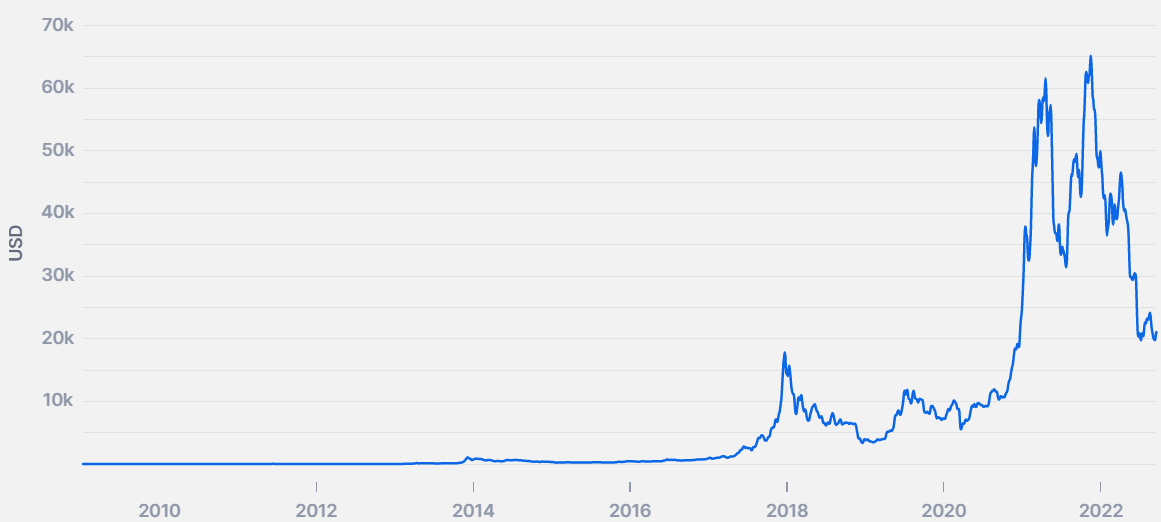
\includegraphics[width=1\textwidth]{pic2}
    \caption{}
    \label{fig:mesh1}
\end{figure}

Также всем криптовалютам присуща медлительность транзакций из-за сложные криптографических вычислений, обеспечивающих их работу. Так, биткойн осуществляет 7 транзакций в секунду, в то время как максимальная производительность платежной системы Visa составляет около 54 тысячи транзакций в секунду. В среднем транзакция в том же биткойне длится порядка 20-30 минут. Этот факт делает криптовалюты крайне неудобными для оплаты физических товаров.\cite{cite8}

Ещё одной проблемой является неразумное использование электроэнергии при эмитировании криптовалют, в особенности тех, в основе которых лежит принцип доказательства выполнения работы. Согласно результатам исследования Кембриджского центра по организации дополнительного финансирования, на биткойн уходит порядка 100 ТВч в год, что соответствует величине, которую потребляют некоторые относительно крупные страны. \cite{cite9}

Но, пожалуй, самой веской причиной не использовать криптовалюты является их статус в законодательстве РФ. На данный момент, использование криптовалют на территории РФ в качестве средства оплаты запрещено, собственно, как и добыча самой валюты.\cite{cite10}


\newpage

\section{Заключение}

В РФ согласно статистике электронные деньги ещё не получили такого обширного распространения как в Европе, что скорее всего связано с недоверием к  новым средствам оплаты.  Так, в частности, самым популярным сервисом, использующим электронные деньги - Яндекс.Деньги пользуются 53 \%,  в то время как, самым популярным банковским сервисом - Сбербанк Онлайн 83 \% населения.\cite[с.~16]{cite3} Что касается криптовалют, то оплата товаров на территории РФ запрещена и правительство, видимо, не собирается менять ситуацию, хотя не исключено, что будет принят новый закон, позволяющий добывать криптовалюту.\cite{cite10} В целом, из-за большого количества недостатков, все ныне существующие криптовалюты крайне затруднительно использовать при оплате физических товаров или накопления сбережений в сравнении с более привычными стандартными деньгами, или централизованными электронными валютами. В данный момент криптовалюты могут иметь только весьма специфическое назначение. 

\newpage

\begin{thebibliography}{99}
	\bibitem{cite1}
		Федеральный закон "О национальной платежной системе" от 27.06.2011 N 161-ФЗ (последняя редакция)
	\bibitem{cite4}
		Кноп К.А. Азы теории чисел. -- 2-е издю, стереотипное -- M.: МЦНМО, 2019. -- 80 с.
	\bibitem{cite2}
		ХабрХабр: Электронные деньги $[$Электронный ресурс$]$ // URL: https://habr.com/ru/post/532062/ (Дата обращения: 12.12.2022)
	\bibitem{cite3}
		Mediascope: как россияне платят онлайн в 2019 году. $[$Электронный ресурс$]$. // \\URL: https://mediascope.net/news/1061511/?sphrase\_id=194741 (дата обращения: 30.11.2022). 
	\bibitem{cite7}
		The Bell: Крах Terra, сбой Tether: что происходит на крипторынке и чем нынешний кризис отличается от прежних $[$Электронный ресурс$]$ // \\URL: https://thebell.io/krakh-terra-sboy-tether-chto-proiskhodit-na-kriptorynke-i-chem-nyneshniy-krizis-otlichaetsya-ot-prezhnikh
	\bibitem{cite8}
		TAdviser: Проблемы блокчейна $[$Электронный источник$]$ // \\URL: https://www.tadviser.ru/index.php
	\bibitem{cite10}
		vc: Легализация криптовалюты в России: тренды и перспективы $[$Электронный источник$]$ // \\ URL: https://vc.ru/u/1304906-crypto-smi/544584-legalizaciya-kriptovalyuty-v-rossii-trendy-i-perspektivy
	\bibitem{cite5}
		 Satoshi Nakomoto Bitcoin: A Peer-to-Peer Electronic Cash System $[$Электронный ресурс$]$ // \\URL: https://bitcoin.org/bitcoin.pdf (Дата обращения: 30.11.2022)
	\bibitem{cite6}
		Yahoo! Finance: 'Only good for drug dealers': More Nobel prize winners snub bitcoin $[$Электронный ресурс$]$ // \\URL: https://finance.yahoo.com/news/good-drug-dealers-nobel-prize-winners-snub-bitcoin-184903784.html
	\bibitem{cite9}
		Cnet: Bitcoin Mining: How Much Electricity It Takes and Why People Are Worried $[$Электронный источник$]$ // \\ URL: https://www.cnet.com/personal-finance/crypto/bitcoin-mining-how-much-electricity-it-takes-and-why-people-are-worried/
\end{thebibliography}

\end{document}
